\chapter{Fundamentals}
\label{cha:Fundamentals}	
This chapter explains the relevant fundamentals necessary for the experiment performed in this research. 

% ✅✅✅✅✅✅
\section{Digital Image Formation}
A digital image is a two-dimensional pixels array(matrix) composed of picture elements. Each pixel represents the numeric representation of the brightness of the corresponding picture element in the x and y-axis. Furthermore, a digital colour image stores colour information for each pixel in three intensity components (channels). A pixel in a colour image represents the value of the combination of three colours Red, Green, and Blue (RGB). Standard formats of storing the colour information are RGB (red, green, blue channels), HSV or HSB (hue, saturation, brightness) and YCbCr (where Y is the luma component, Cb and Cr are the blues and red components relative to the green component). For example, an RGB image supports 16,777,216 different colours because each channel occupies a maximum of 8-bit colour variations (i.e. between 0 and 255). A digital image can be converted from one colour space to another for easy manipulation purposes. 


% ✅✅✅✅✅
\section{Grayscaling}
A grayscale image is a black and white image with shades of grey in-between. There are different techniques for converting a colour image to grayscale. 

\cite{pratt2007digital} developed a color to grayscale image technique using weighted combination of RGB channels in equation \ref{lumi_eqn}. Also, a colour image can be grayscaled using equation \ref{value_eqn} by taking the maximum of the RGB channels \cite{acharya2005image} or taking the average of the three channels \cite{jack2007ntsc} as denoted in equation \ref{inten_eqn}.

\begin{equation} \label{value_eqn}
G_{value} = \max (R,G,B)
\end{equation}

\begin{equation} \label{lumi_eqn}
G_{luminance} = 0.3R + 0.59G + 0.11B
\end{equation}
\begin{equation} \label{inten_eqn}
G_{intensity} = \frac{R +G+B}{3}
\end{equation}
Using grayscale images for extracting descriptors is computationally cheaper and simplifies the algorithm compared to colour images due to working with only one channel (luminance information) as compared to three channels in colour images \cite{kanan2012color}. For example, a 24-bit RGB image becomes 8-bit when converted to grayscale. However, the above mentioned and other colours to grayscale algorithms have different time computation, and appropriate use case scenarios in image recognition tasks \cite{cadik2008perceptual}. According to Kanan and Cottrell \cite*{kanan2012color}, equation \ref{lumi_eqn} is good for object and face recognition tasks.

% ✅✅✅✅✅
\section{Thresholding}
Thresholding is a popular and computationally straightforward technique in computer vision for foreground and background segmentation of images \cite{lee1990comparative}. Thresholding works by converting grayscale images to binary images according to the pixels’ threshold value \cite{nixon2019feature}. This means that each pixel’s brightness/grey value in the interested objects/regions of the input image must be known. The grey values of objects and background can be obtained by drawing a grayscale image histogram.
As the operator of the threshold algorithm goes through every pixel in the image, if the value of the respective pixel is greater than the threshold, it is set to the maximum pixel value (255, i.e. white). On the other hand, if the pixel value is less than the threshold, the value is set to (0, i.e. black). Hence the final image becomes a white and black image showing a segmented region of interest. For example, figure \ref{fig:my_place} shows a thresholded image, where the original image (a) has been transformed into a grayscale image (b), and (c) is a thresholded image where all pixels above the value of 150 are set to 255 and pixels below the threshold value are set to 0. 

\begin{figure}[!htb]
    \centering
    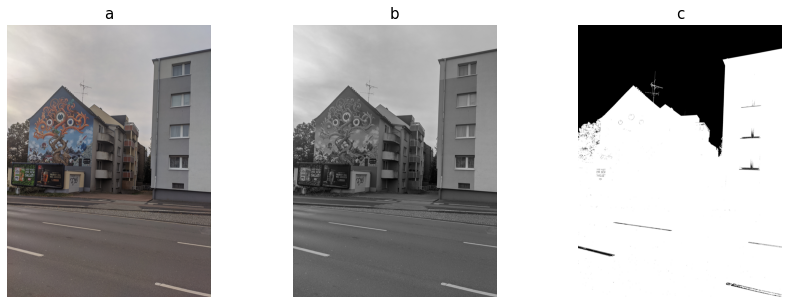
\includegraphics[scale=0.55, keepaspectratio]{Figures/notebook/thresholding.png}
    \caption{(a) Original image (b) Grayscale image (c) Thresholded image.}
    \label{fig:my_place}
\end{figure}  

Sezgin and Sankur \cite{sezgin2004survey} categorises thresholding operators based on the parameters used for manipulating grayscale images into the following six categories.

\begin{itemize}
\item histogram shape-based methods, in this method, the peaks, valleys and curvatures of the smoothed histogram are analysed.
\item clustering-based methods, where the grey-level samples are clustered in two parts as background and foreground objects, or alternately are modelled as a mixture of two Gaussians.
\item entropy-based methods result in algorithms that use the entropy of the foreground and background regions, the cross-entropy between the original and binarised image.
\item object attribute-based methods search a measure of similarity between the grey-level and the binarised images, such as fuzzy shape similarity edge coincidence.
\item the spatial methods use higher-order probability distribution and correlation between pixels.
\item dynamic/local methods adapt the threshold value on each pixel to the local image characteristics.

\end{itemize}

Furthermore, according to Guruprasad \cite{guruprasad2020overview}, the main forms of thresholding methods are:
\begin{itemize}
    \item Threshold Binary
    
    \[
    K(x,y) = \Bigg|_{0 \qquad\quad otherwise}^{maxVal \quad if \quad L(x,y) > threshold}
    \]
    
    \item Threshold Binary, Inverted
    
    \[
    K(x,y) = \Bigg|_{maxVal \qquad\quad otherwise}^{0 \quad if \quad L(x,y) > threshold}
    \]
    
    \item Threshold to zero
    
    \[
    K(x,y) = \Bigg|_{L(x,y) \qquad\quad otherwise}^{0 \quad if \quad L(x,y) > threshold}
    \]
    
    \item Threshold to zero, Inverted
    
    \[
    K(x,y) = \Bigg|_{0 \qquad\quad otherwise}^{L(x,y) \quad if \quad L(x,y) > threshold}
    \]
    
    \item Truncate
    
    \[
    K(x,y) = \Bigg|_{L(x,y) \qquad\quad otherwise}^{threshold \quad if \quad L(x,y) > threshold}
    \]\\
    Where L(x,y) is the source image matrix, K(x,y) is the output image matrix, and maxVal is the maximum pixel value.
\end{itemize}

% ✅✅✅
\subsection*{Otsu’s Thresholding}

The Otsu thresholding method \cite{otsu1979threshold} is named after Nobuyuki Otsu. It is a common thresholding technique for automatically finding the optimal threshold value that gives the best separation between an object and its background for every pixel in the image. Otsu’s thresholding is a clustering-based adaptive thresholding method compared to uniform thresholding forms where the threshold value is manually calculated.
Using Otsu’s method, the optimal threshold $t_{opt}$ is calculated using equation \ref{eu_eqn} by maximising the between-class variance (for class $C_0$ and $C_1$, i.e. background and objects) of the two classes.

\begin{equation} \label{eu_eqn}
\sigma_{B}^{2}(t_{opt}) = \max_{1 \leq k \leq L_{max}} \, \sigma_{B}^{2}(t)
\end{equation}

 The covariance(i.e. between-class variance) is given by 

\begin{equation} \label{e_eqn}
\sigma_{B}^{2}(t) = \frac{{\left[ \mu_T \omega (t) - \mu (t) \right]}^2}{\omega(t) \left[ {1 - \omega(t)} \right] }
\end{equation}


Where t is the threshold, $\mu_T$ is the total mean level of the image, $L_{max}$ is the maximum grey level, $\mu (t)$ and $\omega (t)$ is the zero- and first-order cumulative moments of the normalised histogram up to the threshold level t.

% \subsection{Adaptive Thresholding}
% adaptive mean\\
% adaptive gaussian





% ✅✅✅✅✅✅✅
\section{Gaussian filtering}

In images, smoothing techniques are used to blur out noise and edges that occur due to sampling and processing in the source camera by sliding a kernel of low-pass filter over the image \cite{nixon2019feature}. Noises can occur in images during acquisition, sampling, transmission or processing in the source camera. Examples of noise in images are light fluctuations, sensor noise (camera noise), and quantisation effects. Gaussian smoothing filter is one of the types of image smoothing methods commonly used in computer vision for edge detection due to its optimal performance \cite{basu2002gaussian}.


The Gaussian smoothing operator in 2-D has the form:
\begin{equation} \label{gauss_eqn}
G_{(x,y)} = \frac{1}{2 \pi \sigma^2}e^-{\frac{x^2+y^2}{2\sigma^2}}
\end{equation}
 
Where $\sigma$ is the standard deviation of the distribution and x, y are the values of each pixel in the x, and y coordinate \cite{hsiao2007generic}. The Gaussian function in equation \ref{gauss_eqn} gives the coefficient of the Gaussian kernel, which is slid over an image when smoothing.

% ✅✅✅✅✅✅
\section{Active contours}
Contour is a continuous curve drawn around the edges of detected object/s in an image. The curve traces the exterior outline around objects to be detected at an arbitrary starting point in either a clockwise or an anti-clockwise direction and stops on the boundary of the object \cite{waldchen2018plant}. Drawing contours around objects in an image allows for getting the measurements and angle of orientation of the detected obeject/s, which can be used for other image processing operations like translation and rotation. 



% ✅✅✅✅✅✅
\section{Machine Learning}

Machine learning is a subset of artificial intelligence that uses statistical algorithms to enable computers to learn independently without being explicitly programmed to do so. Machine learning algorithms can be grouped as supervised, unsupervised or reinforcement learning depending on how the algorithm learns the relationships between the input and the expected output data \cite{goodfellow2016deep}. On the other hand, artificial intelligence is a method that trains computers to solve tasks by mimicking the way the human brain works through the use of mathematical and computer science methods.

Furthermore, deep learning is an evolution of machine learning, enabling computers to train themselves in making accurate decisions on tasks through neural networks. 
%Whic trains computers in making accurate decisions on tasks using artificial neural networks

The accuracy of models trained by previously mentioned methods depends heavily on the training dataset’s quality to represent the problem statement adequately. Convolutional neural networks (CNN), deconvolutional neural networks (DNN) and recurrent neural networks (RNN) are common types of deep learning algorithms. This thesis will focus on generative adversarial networks that use CNN and DNN to generate artificial datasets. 
% Figure \ref{} illustrates the relationships between machine learning, artificial intelligence and machine learning using a Venn diagram.

\section{Generative Adversarial Networks (GANs)}
According to \cite{goodfellow2014generative}, “[generative adversarial network is] a new framework for estimating generative models via an adversarial process, in which we simultaneously train two models: a generative model G that captures the data distribution, and a discriminative model D that estimates the probability that a sample came from the training data rather than G; the training procedure for G is to maximise the probability of D making a mistake.” This approach has been successful in generating artificial images in computer vision tasks \cite{denton2015deep}.

To learn a generator distribution $p_g$ over data data $x$, according to \cite{mirza2014conditional} the generator builds a mapping function from a prior noise distribution $p_z(z)$ to data space as $G(z; \theta_g)$. And the discriminator, $D(x; \theta_d)$, outputs a single scalar representing the probability that $x$ came from training data rather than $p_g$. $G$ and $D$ are both trained simultaneously: we adjust parameters for $G$ to minimize $log(1-D(G(z))$ and adjust parameters for $D$ to minimize $logD(X)$, as if they are following the two-player min-max game with value function $V (G, D)$.

\begin{equation} \label{gan_eqn}
\min_G \max_D V(D,G) = E_{x\sim p_{data}(x)}[logD(x)] + E_{z\sim p_z(z)}[log(1-D(G(z)))]
\end{equation}
 Extensions of the GANs architecture includes deep convolutional GANS (DCGANs), conditional GANs (CGAN), information maximising GANs (InfoGANs), amongst others \cite{radford2015unsupervised,chen2016infogan,mirza2014conditional}. Figure \ref{fig:my_gan} shows an overview of the GANs architecture. The architecture begins with a random noise which is inputed to generator for generating fake images. The synthetically generated images are then fed into the discriminator network which also takes original images which fakes ones are generated from as input. The discriminator network determines how close the generated image is to the original image

\begin{figure}[!htb]
    % \centering
    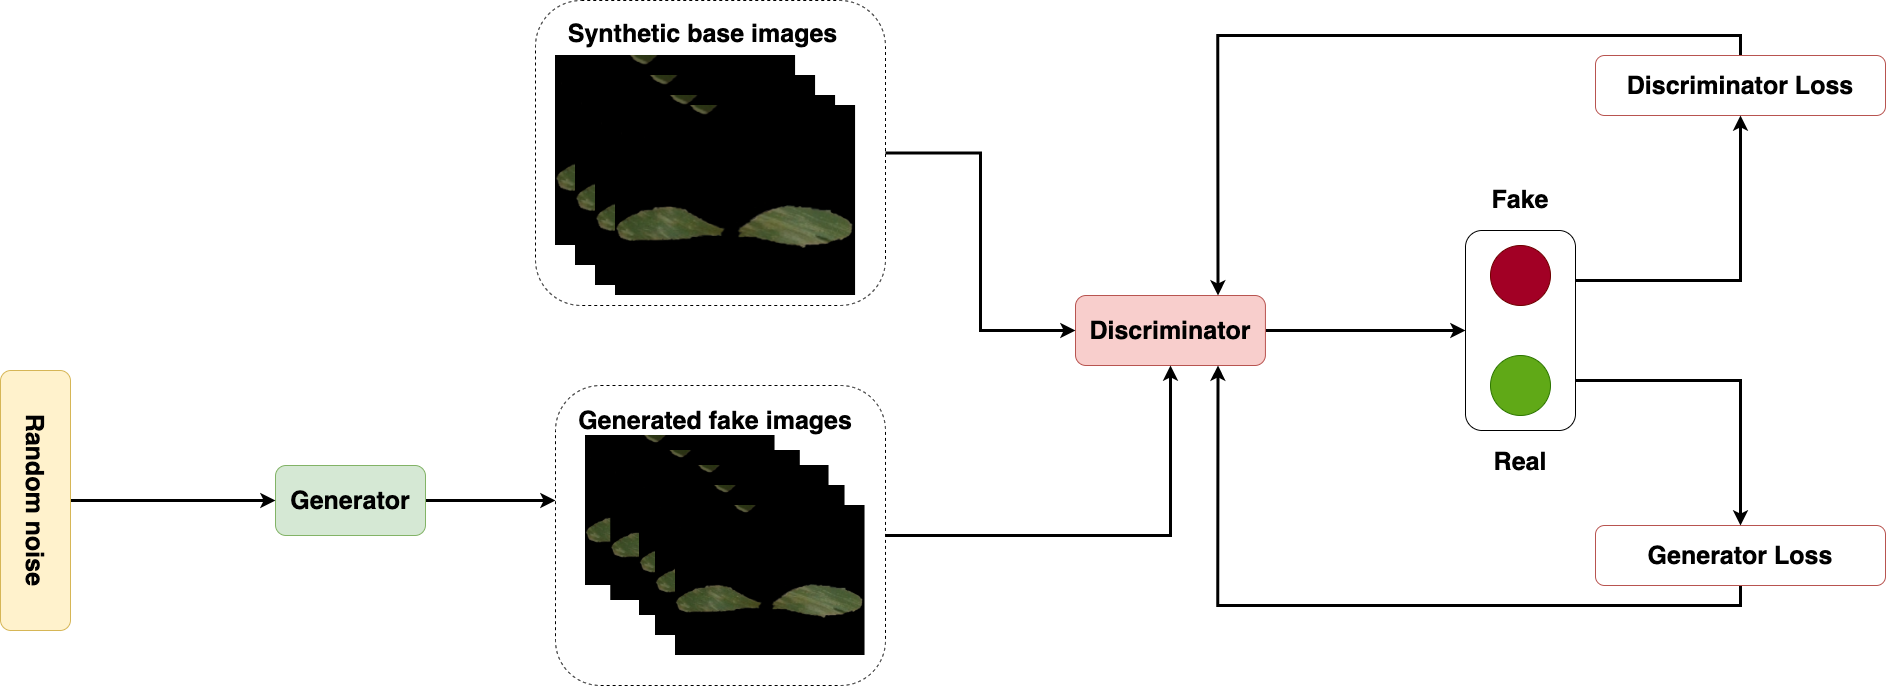
\includegraphics[scale=0.25, keepaspectratio]{Figures/gan.png}
    \caption{Generative adversarial network (GAN) architecture.}
    \label{fig:my_gan}
\end{figure}

Different GAN-based architectures have been developed due to the instability in training models using standard GANs, which often result in ridiculous output by the generator network \cite{radford2015unsupervised}. Therefore, researchers have proposed using other GANs based architectures to create synthetic image datasets to augment currently limited available datasets for training purposes. For example,  Gandhi et al. \cite{gandhi2018plant} used deep convolutional GAN (DCGAN \cite{radford2015unsupervised}) for creating synthetic images to augment the limited number of local images available for training disease detection models for plants in India. Likewise, Barth et al. \cite{barth2020optimising} in their experiment used Cycle GAN for creating 10 500 synthetic images of bell pepper for their segmentation task, Zhu et al. \cite{zhu2018data} created synthetic images from the CVPPP 2017 LSC plant dataset using conditional GAN (CGAN).

% ✅✅✅✅✅
% \section{Plant diseases monitoring in Sugar beet}
% Precision agriculture uses innovative technologies to optimise agricultural production through the use of site-specific management. Particularly in crop production, this aims at crop-specific nutrient deficiencies and disease monitoring, application of fertiliser or pesticides, prediction of yields, automated counting of crops, remote/automatic control of agricultural vehicles like drones and tractors. The underlining principle behind precision farming is to use innovative technologies to economically optimise agricultural production as well as reduce harmful outputs into the environment by applying only the needed amount of fertiliser or pesticides needed during a plantation season \cite{auernhammer2001precision}. Applying the specific amount of resources needed by individual plants will help reduce the impact of chemical by-products or hazardous materials ending up in the environment and economically improve farmers’ financial costs. In other to achieve environmental protection of waters and soils, there is a reduction in the use of fertilisers and pesticides in crop production \cite{otero2005fertiliser}.

% However, the most significant limiting factor in precision farming is the interpretation of collected data from sensors \cite{ondoua2017precision}. Nevertheless, with the current advancement of data manipulation techniques in data science, there is a possibility of addressing these shortcomings to enable a more successful implementation of precision farming.

% % ✅✅✅✅
% \section{Plant disease monitoring in Precision Agriculture}
% In precision farming, plant disease detection is a challenging task, even for professional agronomists and plant pathologists. This complexity in disease detection can be attributed to the fact that there are numerous species of cultivated plants, and there are many causative agents for diseases in each plant. Moreover, in addition to the various diseases affecting plants, plants show variations in visual symptoms to respective diseases. These vast domains of diseases and symptoms frequently cause expert plant pathologists to make wrong disease diagnoses, leading to unjust treatment. Hence the use of optical technologies and computational algorithms for automatic and precise disease detection is invaluable.

% In plants, visual indications of diseases can be seen in leaves, fruits and branches, thereby encouraging the use of optical sensors to assess the different characteristics and parameters in these areas of crops. In the past decades, numerous studies have been conducted on the detection and classification of plant diseases through the combination of feature extraction and machine learning techniques on colour, shapes and texture data from optical sensor systems like spectroscopy, hyperspectral and RGB cameras \cite{xu1996monitoring, hillnhutter2011remote, ramesh2018plant, raza2015automatic}. Currently, researches are geared towards using deep learning-based neural networks with data from optical sensors to create a robust system for the automatic detection of diseases in plants.


% \cite{turkouglu2019plant} in their paper compared the results of using deep feature extractions and transfer learning based on deep learning architectures for disease and pest detection on colour images. They classified the features extracted from the images by neural networks using K-nearest neighbour (KNN), Support vector machine (SVM) and Extreme learning machine (ELM) classifiers. The authors obtained their colour image dataset containing five diseases (Coryneum beijerinckii, Apricot and Peach monilia laxa, Cherry myzus cerasi, Xanthomonas arboricola) and three pests (Erwinia amylovora, Peach sphaerolecanium prunastri, Walnut leaf mite ga) with Nikon 7200d camera during daytime condition on different days in Turkey. There was a total count of 1965 images, which were resized to 224 x 224 pixels and 227 x 227 pixels, and the experiment was conducted with nine different deep learning neural network architectures. They obtained their highest accuracy (97.86\%) with ResNet-50 architecture and SVM classifier. The authors recognised a lower time computation complexity using deep feature extractions architectures than that of transfer learning architectures.

% Likewise, \cite{fuentes2017robust} developed a deep-learning-based method for real-time detection of class and location of 9 different diseases and pests in tomato plants using images captured in-place by camera devices with various resolutions. They conducted their experiment combining deep feature extractors with each of Convolutional Neural Network (Faster R-CNN), Region-based Fully Convolutional Network (R-FCN), and Single Shot Multibox Detector (SSD) architectures. Their datasets contained 5000 images of leaf, stem and fruit captured under different conditions, atmospheric variations and scenarios in greenhouse farms across Korea. They trained and tested their proposed system end-to-end with an Intel Core I7 3.5 GHz Processor on two NVidia GeForce Titan X GPUs. Their experimental results show that the proposed system can effectively recognise diseases and pests despite the complex scenarios in the surrounding plants. The authors highlighted an increase in the performance of their models due to technique-based data annotation and augmentation results.

% \cite{liu2018identification} in their paper presented a novel architecture of a deep convolutional neural network based on AlexNet to detect Mosaic, Rust, Brown spot, and Alternaria leaf spot diseases in apple leaves. In order to avoid the problem of overfitting during the training of their disease recognition model, the authors introduced distortions in their datasets through image rotation and image sharpening processing techniques. The image processing operation increased their total dataset from 1 053 images captured using BM-500GE/BB-500GE digital colour camera in apple experiment station in China to 13 689 images. Their experiment achieved an overall disease detection accuracy of 97.62\% in apple leaves. The results of their experiment indicated that their proposed CNN-based model could accurately identify the four common types of apple leaf diseases with high accuracy and provide a feasible solution for the identification and recognition of apple leaf diseases. Likewise, their approach was found to have a faster convergence rate and reduced number of trainable parameters compared with the standard AlexNet model. However, the authors noted a limiting factor affecting their research domain and many others. They were still scratching the surface in terms of disease detection in apple as it is challenging to gather enough datasets containing all the diseases of apple. 


% \cite{kamal2019depthwise} in their study developed and compared different CNN based architectures with a depthwise separable convolutional network, which has been explicitly incorporated in MobileNet for efficient classification of plant diseases. Their dataset is based on 82,161 simple leaf images containing 55 distinct classes of healthy and diseased plants from the publicly available plant village dataset \cite{hughes2015open}. Their most successful deep learning model architecture, MobileNet, achieved a success rate of 98.65\% with roughly six times lesser parameters than VGG. In addition, reduced MobileNet, a pruned version of MobileNet, with the final five convolution layers retracted, attained similar accuracy compared to MobileNet with substantially reduced parameters.

